\renewcommand{\familydefault}{\sfdefault}

\title{AMVARA DASHBOARD}
\author{
        Amvara Consulting S.L.\\
}
\date{\today} %% Adds today date

\documentclass[12pt]{article}
\usepackage[legalpaper, margin=3cm]{geometry}
\usepackage{hyperref}
\usepackage{graphicx}
\usepackage{fancyhdr}
\graphicspath{ {.images/} }

\begin{document} %% Starts Document
\maketitle %% Prints title and author

\begin{centering} %% Displays an image and webpage url centered
	
\includegraphics{amvara} \par
	\url{https://www.amvara.de} \par
\end{centering}

\newpage %% Page break
\tableofcontents %% Display's Table of contents
\newpage

%%%%%%%%%%%%%%%%%%%%%%%%%%%%%%%%%%%%%%%%%%%%%%%%%%%%%%%%%%%%%%%%
%					  Data Formats Section 					   %
%%%%%%%%%%%%%%%%%%%%%%%%%%%%%%%%%%%%%%%%%%%%%%%%%%%%%%%%%%%%%%%%

\section{Data Formats} %% First Section
Data can be ordered by:
\begin{itemize} %% Unordered List with dots
	\item By Priority [1,2,3,4] Being 1 the most critical and 4 the less critical
	\item By Ticket Type
	\item By Application/Service
	\item By Status
\end{itemize}
\textbf{Note:} All of these can be changed, for example. Instead of Ticket Type, Sales Channel, instead of By priority, by Clothes Size, etc. Everything can be modified according to your needs.\par

\subsection{Dashboard's Main Page}
\noindent
The main page is divided in two parts. First we've got the graphic, it's sorted by ticket type. Next, in the right part (If we are on desktop) or in the bottom part (If we are on mobile) there are 4 tables with monthly information for each data type. It shows the total of each type of data and the percentage\par
\begin{center}
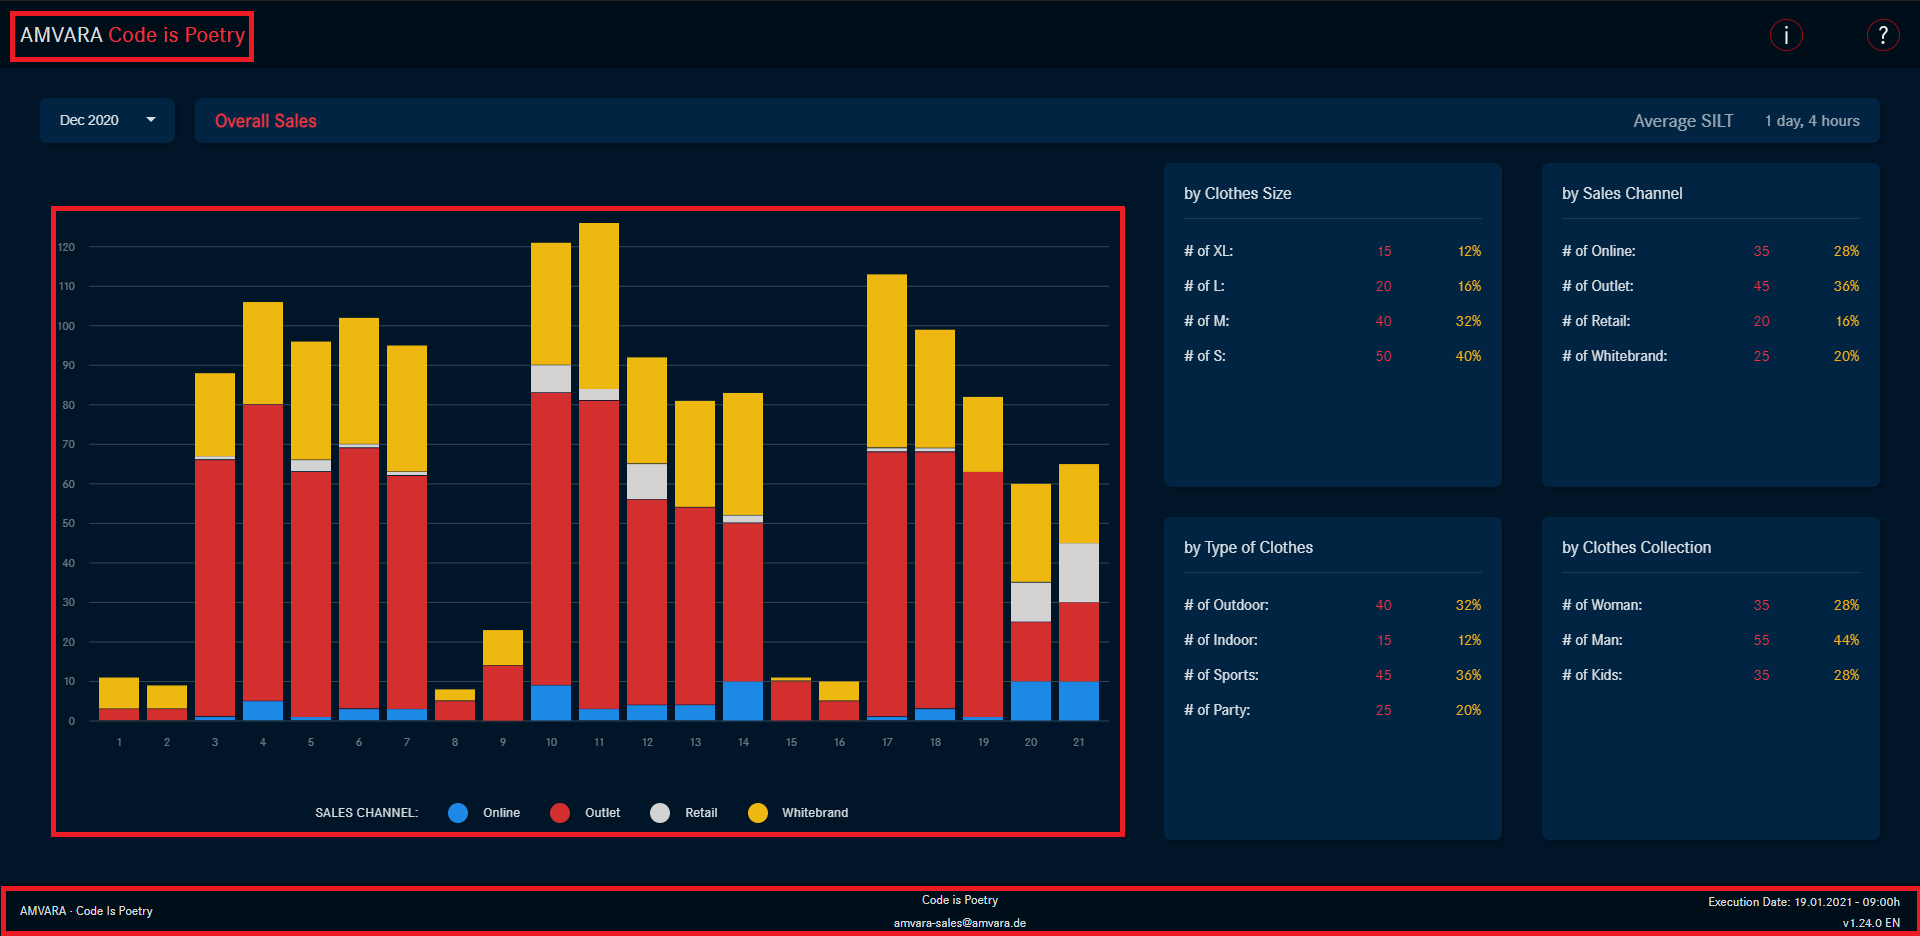
\includegraphics[
  width=440px,
  keepaspectratio,
]{principal}
\end{center}
\newpage %% Page break

%%%%%%%%%%%%%%%%%%%%%%%%%%%%%%%%%%%%%%%%%%%%%%%%%%%%%%%%%%%%%%%%
%					Prepare Skinning Section				   %
%%%%%%%%%%%%%%%%%%%%%%%%%%%%%%%%%%%%%%%%%%%%%%%%%%%%%%%%%%%%%%%%
\newpage
\section{Prepare Skinning} %% Second Section
In this section, we will see how to change the titles, colors and many other things of the dashboard.

\subsection{Header}
Header, is edited in .src/app/components/ux/header/header.component.html, in order to change the title we will edit both span:\par
\begin{center} %% Image Centered
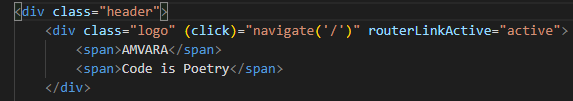
\includegraphics[
  width=300px,
  keepaspectratio,
]{header}
\end{center}

\subsection{Window Title}
Window title is edited in ./src/index.html, in the title element.\par
\begin{center} %% Image Centered
	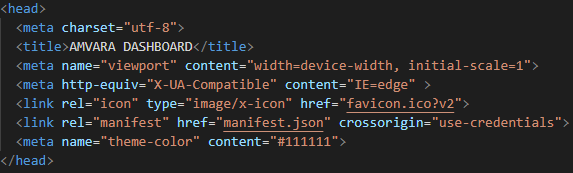
\includegraphics[
	width=300px,
	keepaspectratio,
	]{title}
	\end{center}

\subsection{Loading Screen}
Loading screen title is edited on index.html too, In order to changing the title, edit the content of div class name.\par
\begin{center} %% Image Centered
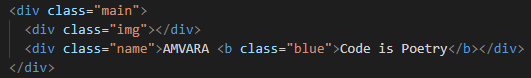
\includegraphics[
	width=300px,
	keepaspectratio,
  ]{loader}
  \end{center}
In order to change the progress bar color, we will edit .progress .progress-value inside index.html styles.\par
\begin{center} %% Image Centered
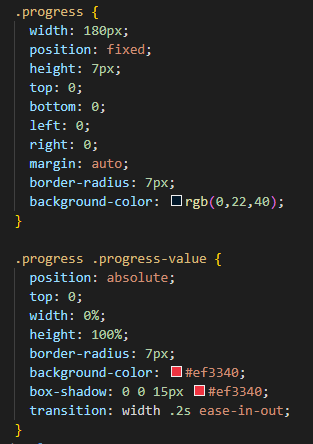
\includegraphics[
	width=200px,
	keepaspectratio,
  ]{loader-css}
  \end{center}
\newpage
  \subsection{General Information}
General information is edited in ./src/assets/config.json. We will have to edit the contact part:\par
\begin{center} %% Image Centered
	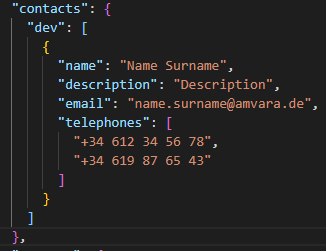
\includegraphics[
		width=200px,
		keepaspectratio,
	  ]{contact}
\end{center}

\subsection{Footer}
Left footer text, is composed by copyright and appTitle, located in the config.json.\par
\begin{center} %% Image Centered
	\includegraphics[
		height=200px,
		keepaspectratio,
	  ]{appTitle}
\end{center}
Mid and right footer text, are edited in .src/app/components/ux/footer/footer.component.html:\par
\begin{center} %% Image Centered
	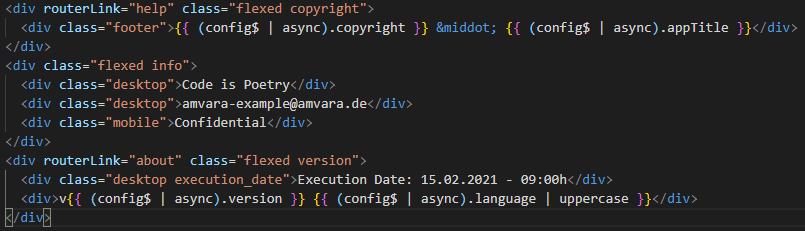
\includegraphics[
		width=400px,
		keepaspectratio,
	  ]{footer-info}
\end{center}
Inside div class flexed, is located the middle text, the text shown will depend if it's accesed from a desktop or a mobile. Then we have the flexed version, that display the execution date and the version of the dashboard.\par
\newpage
\subsection{Colors}
Dasboard's colors, are edited in ./src/app/common/\_colors.scss.\par
\begin{center} %% Image Centered
	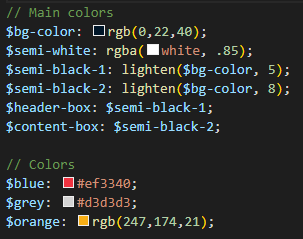
\includegraphics[
	height=150px,
	keepaspectratio,
	]{colors}
\end{center}
The color variables to edit in order to change dashboard colors are:\par
\begin{itemize} %% Unordered List with dots
	\item \$bg-color: Dashboard's background color.
	\item \$semi-white: Dashboard's text color.
	\item \$blue: Dashboard's colors for title and total numbers.
	\item \$grey: General information telephone color.
	\item \$orange: Will change percentage text color and general information link.
\end{itemize}

\subsection{Chart Legend and colors}
In order to change chart legend and colors, the file config.json must be edited. It's located in ./src/assets/config.json\par
\begin{center} %% Image Centered
	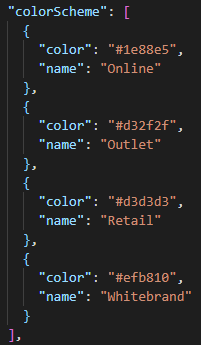
\includegraphics[
	height=250px,
	keepaspectratio,
	]{colorscheme}
\end{center}
Colors are changed in "color" and legend names are changed in "name"\par

%%%%%%%%%%%%%%%%%%%%%%%%%%%%%%%%%%%%%%%%%%%%%%%%%%%%%%%%%%%%%%%%
%				   Introducing Data Section					   %
%%%%%%%%%%%%%%%%%%%%%%%%%%%%%%%%%%%%%%%%%%%%%%%%%%%%%%%%%%%%%%%%
\newpage
\section{Introducing Data} %% Section three \_ \_ of filename.csv needed to print _
The data insertion or edition is done by editing the file Mobile\_List\_Chart.csv (Located in .src/assets/reports/), it's mandatory to use the same name in the ticket type column 
inside the csv and in the colorscheme inside config.json (Located in .src/assets/). If not, when clicking in the bar chart, data will not be displayed correctly.\par

\subsection{dashboardhelper.sh}
Every time Mobile\_List\_Chart.csv is modified, It's important to execute dashboardhelper.sh (Located in .scripts/), this script will read the csv and will complete the other CSV files
such as Mobile\_Tickets\_Priority.csv or Mobile\_Tickets\_Service.csv, among others. it's very simple to run the script, just open a terminal in ./scripts folder and run ./dashboardhelper.sh -m.
For futher information, run ./dashboardhelper -h or ./dashboardhelper --help\par

\subsection{Table Column Names}
In order to change column names to your needs, edit "cell\_header" in the language files inside src/assets/i18n.\par
\begin{center} %% Image Centered
	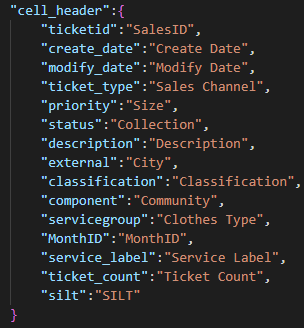
\includegraphics[
	height=220px,
	keepaspectratio,
	]{columns}
\end{center}

\end{document} %% End of document
